% Vertical offsets distinguish workloads within each categorical policy row.
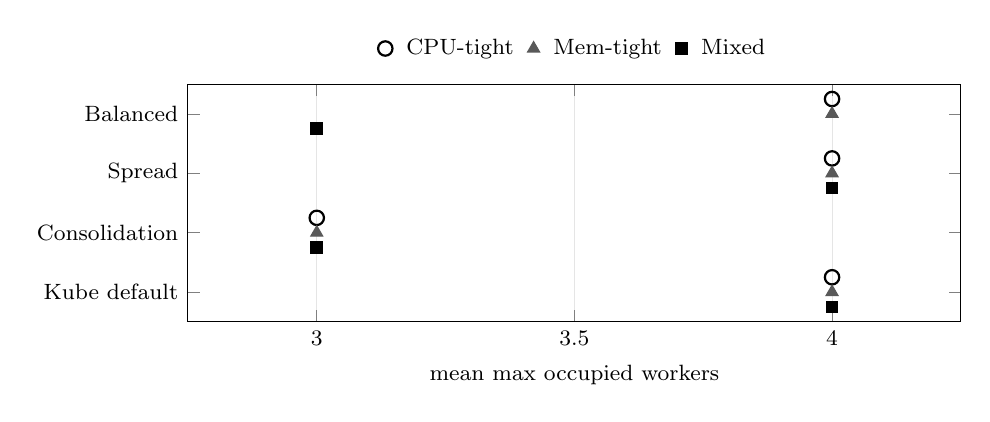
\begin{tikzpicture}
\begin{axis}[
  width=0.94\linewidth, height=4.6cm,
  xmin=2.75, xmax=4.25, xtick={3,3.5,4},
  ymin=0.5, ymax=4.5, ytick={1,2,3,4},
  yticklabels={Kube default,Consolidation,Spread,Balanced},
  tick label style={font=\footnotesize},
  xlabel={mean max occupied workers},
  label style={font=\footnotesize},
  xmajorgrids=true, grid style={gray!20},
  legend style={font=\footnotesize, at={(0.5,1.06)}, anchor=south,
    legend columns=3, column sep=3pt, draw=none, cells={anchor=west}},
]
\addplot[only marks, mark=o, mark size=2.6pt, thick, black]
  coordinates {(4,4.25) (4,3.25) (3,2.25) (4,1.25)};
\addplot[only marks, mark=triangle*, mark size=2.5pt, black!65]
  coordinates {(4,4) (4,3) (3,2) (4,1)};
\addplot[only marks, mark=square*, mark size=2.1pt, black]
  coordinates {(3,3.75) (4,2.75) (3,1.75) (4,0.75)};
\legend{CPU-tight,Mem-tight,Mixed}
\end{axis}
\end{tikzpicture}
